\section{Statistics and numbers}

\begin{description}
	\item[94\%] (130/138 jurisdictions) have made a public commitment to IFRS
	as the single set of global accounting standards.
	\item[83\%](114/138 jurisdictions) already require the use of IFRS by all or most public companies, with most of the remaining jurisdictions permitting their use.
	\item[\$41 trillion] combined GDP of IFRS jurisdictions, representing more than half of the worldwide GDP.
	\item[\$24 trillion non-EU] While the European Union remains the single biggest IFRS jurisdiction, the combined GDP of IFRS jurisdictions outside the EU (US\$24 trillion) is now greater than that of the EU itself (US\$17 trillion).
	\item[50\%]In less than six years since its publication, the IFRS for SMEs has been adopted by 50 per cent (69/138) of jurisdictions while a further 15 jurisdictions are considering doing so.
\end{description}

\begin{figure}[h]
\caption{Requirements}
\centering
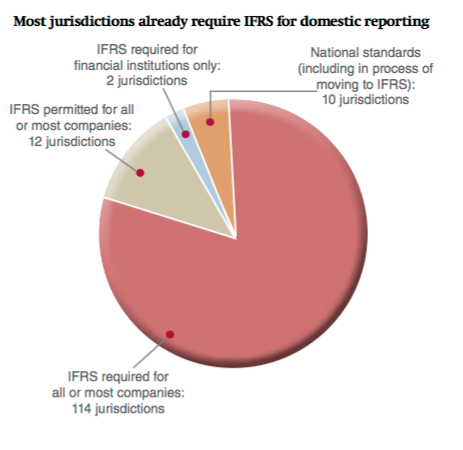
\includegraphics[width=0.8\textwidth]{images/requirements.png}
\end{figure}


\begin{table}[!htb]
\centering
\caption{Number of jurisdictions surveyed}
\label{Number of jurisdictions surveyed}
\resizebox{\textwidth}{!}{%
\begin{tabular}{|l|l|l|l|l|l|}
\hline
\multicolumn{1}{|c|}{\textbf{Regon}} & \multicolumn{1}{c|}{\textbf{In the region}} & \multicolumn{1}{c|}{\textbf{\begin{tabular}[c]{@{}c@{}}That require IRFS \\ for all or most domestic\\  publicly accountable entities\end{tabular}}} & \multicolumn{1}{c|}{\textbf{\begin{tabular}[c]{@{}c@{}}That require IRFS \\ as \% of total \\ jurisdictions in the region\end{tabular}}} & \multicolumn{1}{c|}{\textbf{\begin{tabular}[c]{@{}c@{}}That permit or\\ require IRFS for\\ at least some (but\\ not all or most)\\ domestic publicly\\ accountable\\ entities\end{tabular}}} & \multicolumn{1}{c|}{\textbf{\begin{tabular}[c]{@{}c@{}}That neither\\ require nor permit\\ IRFS for any\\ domestic publicly\\ accountable\\ entities\end{tabular}}} \\ \hline
Europe & 42 & 41 & 98\% & 1 & 0 \\ \hline
Africa & 20 & 16 & 80\% & 1 & 3 \\ \hline
Middle East & 7 & 6 & 86\% & 1 & 0 \\ \hline
Asia-Ocenia & 32 & 24 & 75\% & 3 & 5 \\ \hline
Americas & 37 & 27 & 73\% & 8 & 2 \\ \hline \hline
\textbf{Totals} & \textbf{138} & \textbf{114} & \textbf{83\%} & \textbf{14} & \textbf{10} \\ \hline
\textbf{As \% of 138} & \textbf{100\%} & \textbf{83\%} & \textbf{} & \textbf{10\%} & \textbf{7\%} \\ \hline
\end{tabular}
}
\end{table}